\documentclass[a4paper]{article}

\hoffset=-1in
\voffset=-1in
\textwidth=175mm
\textheight=200mm

\usepackage{amsmath}
\usepackage{graphicx}
\usepackage{multicol}

\begin{document}
    \begin{figure}
        \centering
        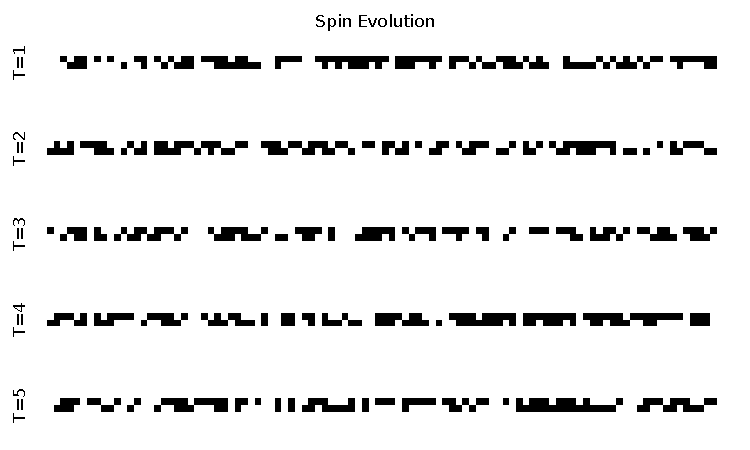
\includegraphics[width=0.5\textwidth]{pub/figures/q1a.pdf}
        \caption{At low temperatures we observed smaller groups of aligned %
            spins. We concluded that the influence of the heat (i.e. %
            \(\tau\sigma\)) on the free energy was low and therefore, that %
            the energy \(U\) was minmised.}
        \label{FIG1}
    \end{figure}

    \begin{multicols}{2}
        Given the partition function \(Z = (2\cosh(\epsilon / \tau))^{N}\), we 
        calculated the internal energy using,
        %
        \begin{align}
            U &= \tau^{2}\partial_{\tau}\ln(Z)\label{EQN1}\\
                &= \tau^{2}\partial_{\tau}
                    \ln\left(2\cosh\left(\frac{\epsilon}{\tau}\right)^{N}\right)
                    \nonumber \\
                &= N\tau^{2}\partial_{\tau}
                    \ln\left(2\cosh\left(\frac{\epsilon}{\tau}\right)\right)
                    \nonumber \\
                &= N\tau^{2}\partial_{\tau}
                    \left(2\cosh\left(\frac{\epsilon}{\tau}\right)\right)
                    \frac{1}{2\cosh\left(\frac{\epsilon}{\tau}\right)}
                    \nonumber \\
                &= N\tau^{2}\partial_{\tau}\left(\frac{\epsilon}{\tau}\right)
                    \frac{\sinh\left(\frac{\epsilon}{\tau}\right)}
                    {\cosh\left(\frac{\epsilon}{\tau}\right)}\nonumber \\
                &= -\epsilon N\tanh\left(\frac{\epsilon}{\tau}\right)
                    \label{EQN2}.
        \end{align}
        %
        We calculated the free energy of the system using,
        %
        \begin{align}
            F &= -\tau\ln Z \label{EQN3}\\
                &= -\tau\ln\left(\left(
                    2\cosh\left(\frac{\epsilon}{\tau}\right)\right)^{N}\right) 
                    \nonumber \\
                &= -N\tau\ln\left(
                    2\cosh\left(\frac{\epsilon}{\tau}\right)\right) 
                    \nonumber \\
                &= -N\tau\ln\left(
                    \exp\left(\frac{\epsilon}{\tau}\right) + 
                    \exp\left(-\frac{\epsilon}{\tau}\right)\right) \nonumber \\
                &= -N\tau\ln\left(\exp\left(\frac{\epsilon}{\tau}\right)
                    \left(1 + \exp\left(-2\frac{\epsilon}{\tau}\right)\right)
                    \right)\nonumber \\
                &= -N\tau\ln\left(\exp\left(\frac{\epsilon}{\tau}\right)\right)
                    - N\tau\ln\left(1 + 
                    \exp\left(-2\frac{\epsilon}{\tau}\right)\right) \nonumber \\
                &= -N\epsilon - N\tau\ln\left(1 + 
                    \exp\left(-2\frac{\epsilon}{\tau}\right)\right)\label{EQN4}. 
        \end{align}
        %
        The entropy followed from the combination of Equation \ref{EQN4} and %
        Equation \ref{EQN2} using Equation \ref{EQN5},
        %
        \begin{align}
            \tau\sigma &= F - U \label{EQN5} \\
                &= -N\epsilon\tanh\left(\frac{\epsilon}{\tau}\right) + 
                    N\epsilon + N\tau\ln\left(1 + 
                    \exp\left(-2\frac{\epsilon}{\tau}\right)\right)\nonumber \\
            \sigma &= \frac{\epsilon}{\tau}\left(1 - 
                    \tanh\left(\frac{\epsilon}{\tau}\right)\right) +
                    \ln\left(1 + \exp\left(-2\frac{\epsilon}{\tau}\right)\right)
                    \label{EQN6}.
        \end{align} 
        %
        Finally, we determined the specific heat using Equation \ref{EQN7} %
        and Equation \ref{EQN2},
        %
        
    \end{multicols}
\end{document}
